
\begin{figure}[htbp]
	\centering
    \graphicspath{{../}}
	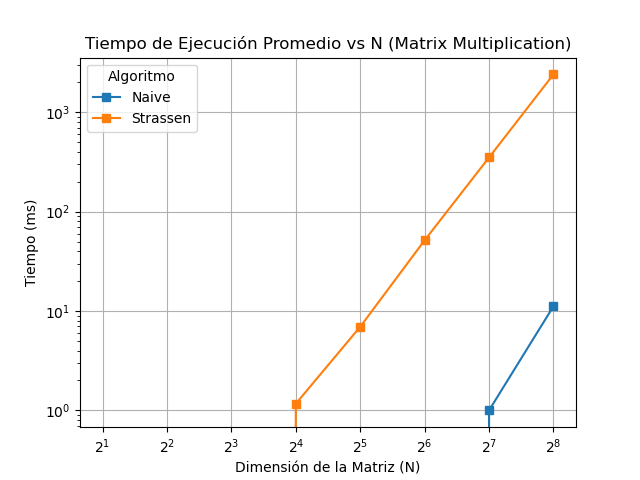
\includegraphics[width=0.8\textwidth]{code/matrix_multiplication/data/plots/matrix_time.png}
	\caption{Tiempo de ejecución vs Dimensión de la matriz para los algoritmos Naive y Strassen.}
	\label{fig:matrix_plot}
\end{figure}

\begin{table}[htbp]
	\centering
	\begin{tabular}{|l|c|c|c|c|c|c|c|c|}
		\hline
		\textbf{Algoritmo} & \textbf{$N=2$} & \textbf{$N=4$} & \textbf{$N=8$} & \textbf{$N=16$} & \textbf{$N=32$} & \textbf{$N=64$} & \textbf{$N=128$} & \textbf{$N=256$} \\ \hline
		Naive & 0.000 & 0.000 & 0.000 & 0.000 & 0.000 & 0.000 & 1.056 & 11.444 \\ \hline
		Strassen & 0.000 & 0.000 & 0.000 & 1.000 & 7.333 & 53.111 & 344.444 & 2312.167 \\ \hline
	\end{tabular}
	\caption{Tiempos de ejecución (en milisegundos) para multiplicacion de matrices. Se observa que el metodo Naive mantiene tiempos inferiores, demostrando el sobrecosto operativo de Strassen en dimensiones previas al umbral de transicion.}
	\label{tab:matrix_time}
\end{table}

\subsection{Multiplicación de Matrices: El peso de las constantes y el umbral empirico}
Como se detalla en la Tabla \ref{tab:matrix_time} y se ilustra en la Figura \ref{fig:matrix_plot}, el algoritmo Naive supera de forma aplastante a Strassen en la practica para las dimensiones evaluadas.  Para la dimension de matriz maxima de N=256, el metodo Naive finaliza en 11.444 ms, mientras que Strassen se dispara a 2312.167 ms. Aunque teóricamente Strassen reduce la cantidad de multiplicaciones escalares de $O(n^3)$ a $O(n^{2.81})$, su sobrecarga estructural y la creacion dinamica de submatrices saturaron la memoria y el procesador antes de que el volumen de datos lograra compensar su costo operativo inicial.

Esto demuestra mediante la experimentacion (empiricamente) que, para dimensiones moderadas, las operaciones directas e iterativas superan a los enfoques de dividir y conquistar teoricos. La regla del límite establece que la funcion con menor orden de crecimiento dominara, pero la constante oculta en la ecuación de recurrencia de Strassen $T(n)=7T(n/2)+O(n^2)$
 es tan alta que el \textit{crossover point} (umbral de transición) donde Strassen se vuelve superior no se alcanza dentro del rango $N \le 256$.

\begin{figure}[htbp]
	\centering
	\graphicspath{{../}}
	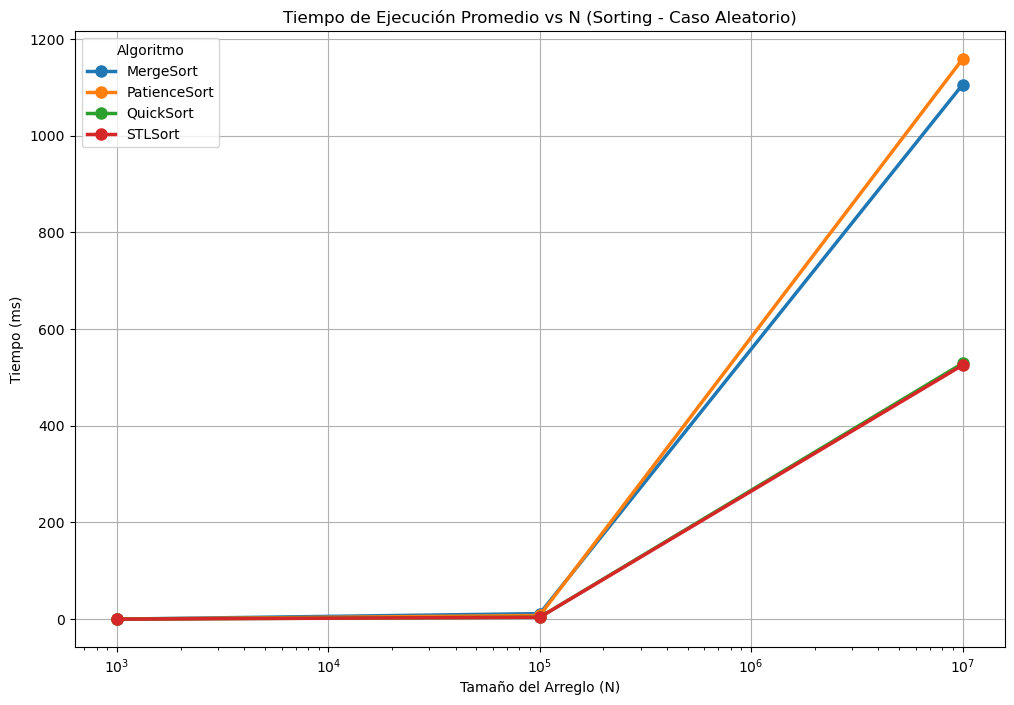
\includegraphics[width=0.8\textwidth]{code/sorting/data/plots/sorting_time.png}
	\caption{Tiempo de ejecución vs Tamaño del arreglo para algoritmos de ordenamiento.}
	\label{fig:sorting_plot}
\end{figure}

\begin{table}[htbp]
	\centering
	\begin{tabular}{|l|c|c|c|}
		\hline
		\textbf{Algoritmo} & \textbf{$N=1000$} & \textbf{$N=100000$} & \textbf{$N=10000000$} \\ \hline
		MergeSort & 0.000 & 0.011 & 1.095 \\ \hline
		PatienceSort & 0.000 & 0.007 & 1.159 \\ \hline
		QuickSort & 0.000 & 0.004 & 0.540 \\ \hline
		STLSort & 0.000 & 0.004 & 0.523 \\ \hline
	\end{tabular}
	\caption{Tiempos de ejecución empíricos (en segundos) para algoritmos de ordenamiento (Distribución Aleatoria).}
	\label{tab:sorting_time}
\end{table}



\subsection{Ordenamiento: Optimización de QuickSort (Antes vs Después)}
\textbf{ºAntes del ajuste:} La implementación original seleccionaba un pivote en el extremo del arreglo, lo que generaba un árbol de recursión completamente desbalanceado al enfrentar datos ascendentes o descendentes. Este peor caso obligaba al algoritmo a ejecutar un número de operaciones cercano a $O(n^ 2)$, volviéndolo tan ineficiente en la práctica como BubbleSort o SelectionSort y provocando tiempos de ejecución excesivos.

\textbf{ºDespués del ajuste:} Al modificar la selección del pivote hacia el centro del subarreglo, permite generar un árbol de recursión balanceado. Esta simple optimizacion ayuda a que se vuelva a un rendimiento promedio del algoritmo a $\Theta(n \log n)$.

Tras la corrección, QuickSort logró ordenar los 10.000.000 de elementos en fracciones de segundo, posicionándose por debajo de las curvas de tiempo respecto a los otros algoritmos.


\subsection{Ordenamiento: Optimización de PatienceSort (Antes vs Después)}

\textbf{Antes del ajuste:} El diseño inicial dependía de búsquedas lineales y eliminaciones directas en el medio de arreglos dinámicos. Eliminar elementos ubicados entre los extremos de una estructura lineal es sumamente ineficiente, requiriendo un tiempo de $O(n)$ en el peor de los casos para desplazar la memoria restante. La repetición de estos desplazamientos degradaba todo el proceso a un tiempo cuadrático $O(n^2)$.  

\textbf{Después del ajuste:} Se implementó una cola de prioridad basada en la estructura de un Min-Heap (priority queue). La teoría respalda que un Heap permite extraer el elemento de máxima prioridad (el mínimo) en un tiempo óptimo de $O(1)$ e insertar nuevos datos reorganizando el árbol en tiempo $O(logn)$.

Reemplazar la búsqueda lineal por búsqueda binaria (lower bound) redujo el costo de inserción, estabilizando el tiempo global de la ejecución a un comportamiento predecible y eficiente de $O(nlogn)$.

\textbf{Observacion: AL ejecutar el sorting.cpp el cual ejecutaba todos los algoritmos, hice un intento considerando las versiones no optimizadas de QuickSort y PatienceSort, lo deje andando por 12 horas y al despertarme aun seguia andando, por lo que decidi analizar sus versiones optimizadas.}

\subsection{Ordenamiento: STLSort y el poder de los algoritmos híbridos}
Al observar la Tabla \ref{tab:sorting_time}, destaca que \texttt{STLSort} (la implementación estándar del lenguaje) obtiene el mejor rendimiento general para $N=10^7$
con 0.523 segundos, superando ligeramente al QuickSort optimizado (0.540 segundos). Esta ventaja radica en que las bibliotecas estándar modernas implementan algoritmos híbridos, comúnmente \textit{IntroSort}. Este enfoque comienza ejecutando QuickSort para aprovechar su velocidad promedio, pero si detecta que la profundidad de recursión excede 2logn, cambia dinámicamente a HeapSort para garantizar un peor caso de $O(nlogn)$, y utiliza InsertionSort para subarreglos muy pequeños donde las constantes operativas son más bajas. La estabilización geométrica en la Figura \ref{fig:sorting_plot} confirma la superioridad técnica de no depender de una sola estrategia de ordenamiento.

\subsection{Impacto de la Localidad de Caché (Cache Locality)}
Un factor determinante que la notación teorica Big-O ignora es la interacción con la arquitectura de memoria del hardware. QuickSort y STLSort procesan los datos \textit{in-place} mediante punteros que avanzan secuencialmente. Esto genera una alta \textit{localidad espacial}, permitiendo que el procesador cargue bloques contiguos de datos en la memoria caché (L1/L2) minimizando los tiempos de busqueda.

Por el contrario, algoritmos como PatienceSort, a pesar de su optimización con Min-Heap, fragmentan el acceso a la memoria. Como se evidencia en la Tabla \ref{tab:sorting_time}, PatienceSort es el algoritmo más lento para $N=10^7$
(1.159 s). La necesidad de saltar constantemente entre distintos nodos del Heap y las cimas de multiples pilas dinamicas (vectores) destruye la localidad de caché, forzando a la CPU a buscar datos en la memoria RAM principal repetidamente.


\subsection{Consumo Espacial: Sobrecarga en la mezcla y estructuras}A pesar de que MergeSort, PatienceSort y QuickSort comparten una complejidad temporal eficiente, la Tabla \ref{tab:sorting_time} ubica a los dos primeros con tiempos absolutos superiores al segundo. Esta brecha ocurre por el manejo de la memoria extra.MergeSort exige la creación de arreglos auxiliares en cada nivel de recursión, sumando exactamente $2n$ (obtenido mediante el stack de recursion) asignaciones físicas para trasladar elementos, generando un costo estricto de memoria adicional de $O(n)$. PatienceSort sufre una penalización similar por instanciar múltiples arreglos dinámicos para sus colas. QuickSort opera aislando intercambios directamente sobre las direcciones originales, manteniendo una huella extra mínima de $O(\log n)$ (exclusiva de los llamados en la pila de ejecución recursiva), lo que alivia el trabajo del administrador de memoria del sistema y acelera el tiempo absoluto de ejecución.


\subsection{Estabilidad vs Rendimiento}
A pesar de la evidente superioridad en la ecperimentacion(empirica) de QuickSort y STLSort en términos de tiempo de ejecución y consumo espacial(memoria), existe un factor teórico crítico que no se refleja en las gráficas de rendimiento absoluto: la \textit{estabilidad} del algoritmo. 

Un algoritmo de ordenamiento es estable si garantiza que los elementos con claves identicas mantendrán su orden relativo original tras el procesamiento. MergeSort es un algoritmo inherentemente estable gracias a la forma secuencial en que mezcla los subarreglos. Por el contrario, el enfoque \textit{in-place} de QuickSort, debido a sus intercambios dinámicos, es inestable. De igual manera, PatienceSort (al extraer cimas desde el Min-Heap) y la implementacion estandar de \texttt{STLSort} (basada en IntroSort) carecen de estabilidad. De hecho, cuando el desarrollo en C++ requiere conservar el orden relativo, se debe sacrificar la velocidad pura de \texttt{std::sort} y utilizar explícitamente \texttt{std::stable\_sort} (cuya implementación suele basarse precisamente en MergeSort).

Este atributo es fundamental. En contextos donde los registros poseen múltiples campos y requieren ordenamientos encadenados (por ejemplo, ordenar una base de datos de pacientes primero por fecha de ingreso y luego por prioridad medica), la estabilidad es un requerimiento necesario. En estos escenarios, el costo adicional de $O(n)$ en memoria y el ligero incremento en los tiempos de ejecución que presenta MergeSort dejan de ser una desventaja, convirtiéndose en el precio necesario a pagar para mantener la integridad relacional de los datos. Esto demuestra que la elección del algoritmo óptimo no depende únicamente de la velocidad pura, sino de las restricciones del dominio del problema.